\documentclass[12pt,a4paper]{article}
\usepackage{amsmath, amssymb, graphicx}
\usepackage{geometry}
\geometry{a4paper, margin=1in}

\begin{document}

\begin{titlepage}
\centering
\vspace*{3cm}
{\LARGE \textbf{ME302: 2024-25 - II} \par}
\vspace{1cm}
{\LARGE \textbf{COURSE PROJECT REPORT} \par}
\vspace{2cm}
{\Large Harish (220423), Deepavath Raghu Ram Naik (220333), Krishna Prajapati (220548)\par}
\end{titlepage}

\section*{PROBLEM DESCRIPTION}
The objective of this project is to develop and test a scaled model of a turbomachine component that will ultimately be incorporated into a future gas turbine engine. The full-size prototype has a characteristic length of 0.2 meters. In order to analyze its performance, the component must be tested in a smaller, high-pressure, closed-loop test facility.

Two major constraints, however, must be kept in mind during testing:
\begin{itemize}
    \item The highest pressure at any point in the facility should not exceed 250 kPa.
    \item The exit stagnation pressure ($P_{05}$) should be equal to or higher than the inlet stagnation pressure ($P_{01}$) for continuous closed-loop operation.
\end{itemize}

Besides meeting these requirements, the scaled model should have similarity of flow conditions with the prototype. More precisely, both the Mach number (target value = 0.55) and Reynolds number (target value = $3 \times 10^6$) should be replicated. The challenge is to determine the largest possible scale (model size divided by prototype size) that meets both the similarity of flow and facility constraints.

\section*{METHODOLOGY}
In order to solve the problem, a step-by-step procedure was employed:

\subsection*{Create Flow Similarity}
Isentropic flow and ideal gas behavior equations were utilized to correlate the flow characteristics such as pressure, temperature, density, and velocity at various locations within the system.

\subsection*{Mass Flow Rate Modeling}
The real mass flow rate was modeled in terms of a reference mass flow rate and the ratio of stagnation conditions through a general scaling formula.

\subsection*{Reynolds Number Matching}
The Reynolds number equation (Re = $\frac{\rho C L}{\mu}$) was used to match the dynamic conditions of the model with the prototype. This yielded one of the geometrical scale constraints.

\subsection*{Facility Constraints}
For each scale considered, the corresponding pressures at different stations (particularly $P_{02}$, $P_{04}$, and $P_{05}$) were determined to ensure that:
\begin{itemize}
    \item No component of the system exceeds 250 kPa.
    \item The flow remains closed-loop ($P_{05} \geq P_{01}$).
\end{itemize}

\subsection*{Calculate Feasible Scale}
With the relations and constraints provided above, the maximum feasible geometric scale was calculated.

\subsection*{Software and Tools}
Python was utilized throughout the analysis. Computations included fluid property calculations, scaling relations, and checks for constraints. Compressor map data were used to ensure that the operating point of the selected scale falls within acceptable bounds.

This technique ensured that the selected scale maintained flow similarity while adhering to the safe operating ranges of the test facility.

\section*{RESULTS AND DISCUSSION}

\subsection*{Mass Flow Rate Relation}
\begin{align*}
\dot{m} &= \rho_4 A_4 C_4 \\
\dot{m} &= \dot{m}_{ref} \left( \frac{P_{01}}{101.325 \times 10^3} \right) \left(\sqrt{\frac{T_{01}}{293}}\right) = \frac{\rho_4 \pi D_4^2 C_4}{4} \\
D_4 &= 2 \cdot L_{model} \Rightarrow A_4 = \pi L_{model}^2 \\
\Rightarrow \dot{m} &= \dot{m}_{ref} \left( \frac{P_{01}}{101.325 \times 10^3} \right) = \rho_4 \pi L_{model}^2 C_4 \tag{1}
\end{align*}
\noindent Where $\rho_4 = \frac{P_4}{RT_4}$

\subsection*{Temperature at Station 4 ($T_4$)}
\begin{align*}
\frac{T_{02}}{T_4} &= 1 + \frac{(\gamma - 1)}{2} M^2 = 1 + (1.4 - 1) \cdot \frac{(0.55)^2}{2} = 1.0605 \\
T_4 &= \frac{T_{02}}{1.0605} \tag{2}
\end{align*}

\subsection*{Pressure at Station 4 ($P_4$)}
\begin{align*}
\frac{P_{04}}{P_4} &= \left(1 + \frac{(\gamma - 1)}{2} M^2 \right)^{\frac{\gamma}{\gamma - 1}} = 1.228 \tag{3}
\end{align*}
\noindent Given:
\begin{align*}
\Delta P_{023} &= P_{02} - P_{03} = 0.015 P_{02} \Rightarrow P_{03} = 0.985 P_{02} \\
\Delta P_{045} &= P_{04} - P_{05} = 0.05 P_{04} \Rightarrow P_{05} = 0.95 P_{04} \\
P_{03} &= P_{04} \Rightarrow P_{04} = 0.985 P_{02} \tag{4} \\
\Rightarrow P_4 &= \frac{P_{04}}{1.228} = 0.8021 P_{04}
\end{align*}

\subsection*{Velocity at Station 4 ($C_4$)}
\begin{align*}
T_{04} &= T_4 + \frac{C_4^2}{2 C_p} \\
C_p &= \frac{\gamma R}{\gamma - 1} = \frac{1.4 \cdot 287}{0.4} = 1004.5 \\
T_{02} \left(1 - \frac{1}{1.0605} \right) &= \frac{C_4^2}{2 C_p} \\
\Rightarrow C_4 &= \sqrt{114.611 \cdot T_{02}} \tag{5}
\end{align*}

\subsection*{Density at Station 4 ($\rho_4$)}
\begin{align*}
\rho_4 &= \frac{P_4}{RT_4} = \frac{0.8021 P_{02} \cdot 1.0605}{T_{02} \cdot 287} = \frac{2.9638 \cdot 10^{-3} P_{02}}{T_{02}} \tag{6}
\end{align*}

\subsection*{Solving for $L_{model}$}
\begin{align*}
\text{From Eqns. (1), (5), and (6):} \\
\dot{m}_{ref} \left(\frac{P_{01}}{101.325 \cdot 10^3}\right) &= \frac{2.9638 \cdot 10^{-3} \cdot P_{02} \cdot \pi \cdot L_{model}^2 \cdot C_4}{T_{02}} \\
L_{model}^2 &= \dot{m}_{ref} \cdot \sqrt{\frac{T_{02}}{T_{01}}} \cdot \frac{1}{(P_{02}/P_{01})} \cdot 589.759 \\
&= \dot{m}_{ref} \cdot \sqrt{\frac{T_0ratio}{P_0ratio}} \cdot 589.759 \\
\Rightarrow L_{model} &= \sqrt{\frac{\dot{mref}}{P_0ratio}} \cdot T_0ratio^{1/4} \cdot 0.0412
\end{align*}

\subsection*{Scale Determination}
\begin{align*}
\text{Scale} &= \frac{L_{model}}{L_{prototype}} = \sqrt{\frac{\dot{m}ref}{P_0ratio}} \cdot T_0ratio^{1/4} \cdot \frac{0.0412}{0.2} = \sqrt{\frac{\dot{m}}{P_0ratio}} \cdot T_0ratio^{1/4} \cdot 0.206
\end{align*}

\noindent Maximum scale from compressor map = 0.619 \\
Data Point: 
\begin{align*}
\dot{m}_{ref} &= 10.55028375 \tag{7} \\
P_0 \text{ ratio} &= 1.210453952 \tag{8} \\
T_0 \text{ ratio} &= 1.068519008 \tag{9}
\end{align*}

\subsection*{Reynolds Number Relation}
\begin{align*}
Re &= \frac{\rho_4 C_4 L_{model}}{\mu_4} \tag{10} \\
\rho_4 &= \frac{\dot{m}}{A_4 C_4} = \frac{\dot{m}}{\pi D_4^2 C_4} = \frac{\dot{m} P_{01}}{318.322 \cdot 10^3 C_4 L_{model}^2} \tag{11}
\end{align*}

\begin{align*}
\text{Given: } Re = 3 \times 10^6, \mu_4 = 1.83 \times 10^{-5} \\
\Rightarrow L_{model} &= \frac{\dot{m}_{ref} P_{01}}{17.476 \cdot 10^6}
\end{align*}

Using $L_{model} = \text{scale} \cdot L_{prototype} = 0.619 \cdot 0.2 = 0.1238$ m:
\begin{align*}
0.1238 &= \frac{10.55028375 \cdot P_{01}}{17.476 \cdot 10^6} \\
\Rightarrow P_{01} &= 205.068~\text{kPa} \tag{12}
\end{align*}

\subsection*{Pressure Calculations}
\begin{align*}
P_{02} &= 1.210453952 \cdot P_{01} = 248.225~\text{kPa} \tag{13} \\
P_{04} &= 0.985 \cdot P_{02} = 244.502~\text{kPa} \\
P_{05} &= 0.95 \cdot P_{04} = 232.277~\text{kPa}
\end{align*}

\subsection*{Constraints Check}
\begin{itemize}
  \item $P_{05} = 232.277$ kPa $> P_{01} = 205.068$ kPa \hfill \
  \item maximum allowable pressure, $P_{02} = 248.225$ kPa $< 250$ kPa \hfill \
\end{itemize}

\section*{Discussion}

\begin{figure}[h!]
    \centering
    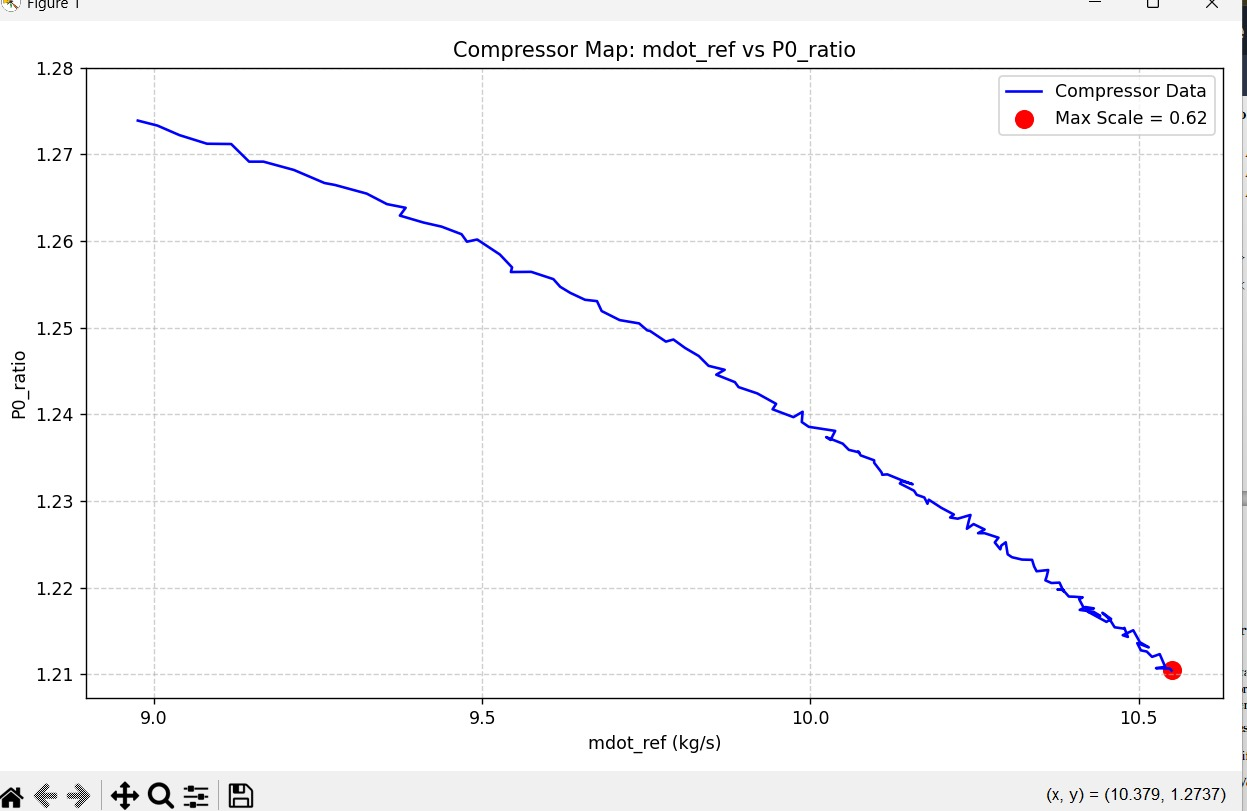
\includegraphics[width=0.75\textwidth]{Compressor Map mdot_ref vs P0_ratio.jpg}
    \caption{Compressor operation map (P\(0\) ratio vs. \(\dot{m}{\text{ref}}\)) showing the 
    chosen operating point in red.}
    \label{fig:comp_map}
\end{figure}

The graph illustrates the compressor performance with \texttt{mdot\_ref} on the x-axis and \texttt{P0\_ratio} on the y-axis. A clear downward trend is observed, where increasing the mass flow rate results in a gradual drop in pressure ratio. The curve reflects stable operation with minimal fluctuations, except near the highest flow rate. The red marker highlights the point where the scale value is maximum, indicating a performance peak. This point could be useful for identifying the most efficient operating condition of the compressor.




\section*{FUTURE WORK}

\subsection*{1. Smarter Diffuser Shapes for Better Performance}

\textbf{The Challenge:} \\
Diffusers act as the "exit ramps" for airflow in turbomachinery. Poorly designed shapes can result in flow separation or take up excessive space, leading to energy losses. The aim is to identify an optimal diffuser angle that balances compactness with aerodynamic efficiency.

\vspace{0.5em}

\textbf{How We Plan to Test This:}
\begin{itemize}
    \item Fabricate multiple diffuser geometries with angles ranging from $5^\circ$ to $15^\circ$.
    \item Use Particle Image Velocimetry (PIV) systems to visualize and analyze airflow behavior.
    \item Validate results through Computational Fluid Dynamics (CFD) simulations.
\end{itemize}

\vspace{0.5em}

\textbf{Industry Relevance:}
\begin{itemize}
    \item Energy firms could achieve 2--3\% compressor efficiency improvements, resulting in substantial cost savings.
    \item Aerospace companies (e.g., Pratt \& Whitney) are continuously seeking more compact and efficient designs.
\end{itemize}

\vspace{0.5em}

\textbf{Real-World Examples:}
\begin{itemize}
    \item NASA's report \#TP-2005-213934 outlines similar diffuser optimization research.
    \item Modern wind turbine technology also benefits from enhanced diffuser designs to increase power output.
\end{itemize}

\vspace{1em}

\subsection*{2. Active Airflow Control Systems}

\begin{figure}[h!]
    \centering
    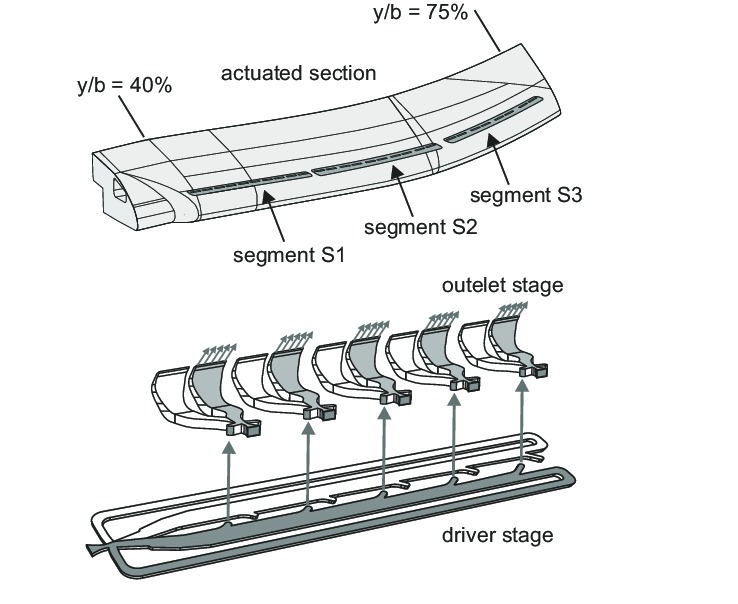
\includegraphics[width=0.75\textwidth]{image1.jpg}
    \caption{Active Airflow Control Systems}
    \label{fig:comp_map}
\end{figure}

\textbf{The Big Idea:} \\
Introduce dynamic control systems that adjust airflow actively using jets or vibrating surfaces—similar to how sails are continuously adjusted on a boat.

\vspace{0.5em}

\textbf{Proposed Implementation:}
\begin{itemize}
    \item Embed miniature air injectors in the test section.
    \item Experiment with various pulsing frequencies and patterns.
    \item Use high-sensitivity pressure sensors to quantify flow improvements.
\end{itemize}

\vspace{0.5em}

\textbf{Potential Applications:}
\begin{itemize}
    \item Enhance jet engine performance in turbulent or unsteady conditions.
    \item Minimize wear and tear in power plants by ensuring uniform flow profiles.
\end{itemize}

\textbf{Cutting-Edge Context:}
\begin{itemize}
    \item Techniques similar to these are patented by companies like GE (e.g., US20180023421A1).
    \item However, this research seeks to develop simpler and more cost-effective alternatives.
\end{itemize}











\subsection*{3. Tougher Materials for Harsh Conditions}

\begin{figure}[h!]
    \centering
    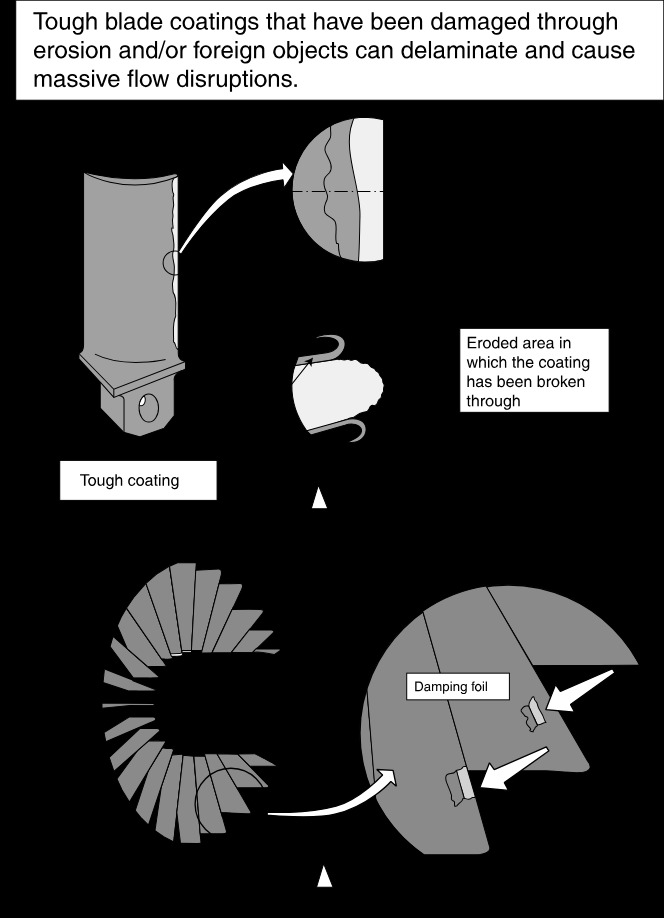
\includegraphics[width=0.75\textwidth]{image2.jpg}
    \caption{Tougher Materials for Harsh Conditions}
    \label{fig:comp_map}
\end{figure}

\textbf{The Problem:} \\
Turbomachinery components are exposed to extreme environments, including sand, muddy water, and other particulates—similar to driving through a sandstorm daily.

\vspace{0.5em}

\textbf{Our Proposed Solution:}
\begin{itemize}
    \item Test advanced materials such as 3D-printed titanium alloys and ceramic coatings.
    \item Simulate real-world wear using controlled dirty flow test setups.
\end{itemize}

\vspace{0.5em}

\textbf{Target Industries:}
\begin{itemize}
    \item Oil and gas operations in desert conditions.
    \item Hydropower plants affected by sediment-rich water sources.
\end{itemize}

\vspace{0.5em}

\textbf{Supporting Evidence:}
\begin{itemize}
    \item Coatings can extend component lifespan by up to three times (\textit{Wear Journal}, 2019).
    \item Testing will follow adapted procedures based on ASTM G76 standards for erosion testing.
\end{itemize}









\subsection*{Required Python Libraries}
\begin{itemize}

    \item \texttt{pandas:}--for reading and handling tabular data
    \item \texttt{matplotlib:}--for plotting graphs
    \item \texttt{numpy:}--for numerical operations
    
\end{itemize}
 If you do not have these packages installed, you can install them using pip (Python’s package
 manager). Open your terminal or command prompt and execute the following command:
 
                pip install pandas numpy matplotlib
                
\textbf{Here are some things that should be in mind:-}
\begin{enumerate}
    \item A Python script is a file with a \texttt{.py} extension that contains Python code.

    \item It runs step by step to perform tasks like reading data, doing calculations, or showing plots.

    \item The data file it uses (like \texttt{Compressor\_operation\_map.txt}) should be in the same folder as the script unless you give the full file path.

    \item You can run the script by typing \texttt{python script\_name.py} in a terminal or Python environment.
\end{enumerate}

\begin{thebibliography}{9}

\bibitem{ref1}
NASA Technical Paper Available: \url{https://ntrs.nasa.gov/citations/20050172494}

\bibitem{ref2}
GE Patent (US20180023421A1):
\url{https://patents.google.com/patent/US20180023421A1/}

\bibitem{ref1}
Wear Journal (2019) Coatings Study: \url{https://www.sciencedirect.com/science/article/abs/pii/S0043164818317353}
\end{thebibliography}

\end{document}
